\documentclass[10pt,twocolumn,letterpaper]{article}

\usepackage{cvpr}
\usepackage{times}
\usepackage{epsfig}
\usepackage{graphicx}
\usepackage{amsmath}
\usepackage{amssymb}
\usepackage[utf8]{inputenc}
\usepackage{fullpage}
\usepackage{subfig}

\usepackage[margin=1in]{geometry} 
\usepackage{amsmath,amsthm,amssymb}
 
\newcommand{\N}{\mathbb{N}}
\newcommand{\Z}{\mathbb{Z}}
 
\newenvironment{theorem}[2][Theorem]{\begin{trivlist}
\item[\hskip \labelsep {\bfseries #1}\hskip \labelsep {\bfseries #2.}]}{\end{trivlist}}
\newenvironment{lemma}[2][Lemma]{\begin{trivlist}
\item[\hskip \labelsep {\bfseries #1}\hskip \labelsep {\bfseries #2.}]}{\end{trivlist}}
\newenvironment{exercise}[2][Exercise]{\begin{trivlist}
\item[\hskip \labelsep {\bfseries #1}\hskip \labelsep {\bfseries #2.}]}{\end{trivlist}}
\newenvironment{reflection}[2][Reflection]{\begin{trivlist}
\item[\hskip \labelsep {\bfseries #1}\hskip \labelsep {\bfseries #2.}]}{\end{trivlist}}
\newenvironment{proposition}[2][Proposition]{\begin{trivlist}
\item[\hskip \labelsep {\bfseries #1}\hskip \labelsep {\bfseries #2.}]}{\end{trivlist}}
\newenvironment{corollary}[2][Corollary]{\begin{trivlist}
\item[\hskip \labelsep {\bfseries #1}\hskip \labelsep {\bfseries #2.}]}{\end{trivlist}}
 


% Include other packages here, before hyperref.

% If you comment hyperref and then uncomment it, you should delete
% egpaper.aux before re-running latex.  (Or just hit 'q' on the first latex
% run, let it finish, and you should be clear).
\usepackage[breaklinks=true,bookmarks=false]{hyperref}

\cvprfinalcopy % *** Uncomment this line for the final submission

\def\cvprPaperID{****} % *** Enter the CVPR Paper ID here
\def\httilde{\mbox{\tt\raisebox{-.5ex}{\symbol{126}}}}

% Pages are numbered in submission mode, and unnumbered in camera-ready
%\ifcvprfinal\pagestyle{empty}\fi
\setcounter{page}{1}
\begin{document}

%%%%%%%%% TITLE
\title{Clasificadores PHOW}

\author{Francisco J. Cedano\\
Departamento de Ingenier\'ia Biom\'edica\\
Universidad de Los Andes\\
{\tt\small fj.cedano803@uniandes.edu.co}
% For a paper whose authors are all at the same institution,
% omit the following lines up until the closing ``}''.
% Additional authors and addresses can be added with ``\and'',
% just like the second author.
% To save space, use either the email address or home page, not both
}%\and
%Second Author\\
%Institution2\\
%First line of institution2 address\\
%{\tt\small secondauthor@i2.org}


\maketitle
%\thispagestyle{empty}

%%%%%%%%% ABSTRACT
\begin{abstract}
   En el presente laboratorio se estudian métodos para reconocimiento imágenes en categorías respectivas usando la base de datos caltech101 y la base de datos imagenet-tiny, esta segunda contiene imágenes de mayor complejidad. Los métodos usados se basan en PHOW (descriptores SIFT multi-escala. En este trabajo se variaron diferentes variables en el método, con el fin de estimar la exactitud de los métodos y el costo computacional.
   
\end{abstract}

%%%%%%%%% BODY TEXT
\section{Introducción}

Se usaron dos diferentes bases de datos en este proyecto. La primera es caltech101 (ver Figura 1.) la cual contiene 101 clases de objetos [1], tales como: elefantes, computadores personales, ventiladores, etc. Son cerca de 40 a 800 imágenes por categoría. La mayoría tiene cerca de 50 imágenes. El tamaño de cada imagen es de aproximadamente 300x200 píxeles. Por otro lado, también se usó la base de datos de imagenet-tiny (ver Figura 1.)[2], tiene 200 clases de objetos, 100 imágenes por clases de 256x256 píxeles. Imagenet-tiny es una base de datos de difícil clasificación por su aleatoriedad en las imágenes. La gran diferencia entre ambas bases de datos es la variabilidad de las imágenes dentro de cada categoría en imagenet-tiny, dado que en Caltech101 no tienen cambios de deformación, luminosidad, puntos de vista, etc. 

\begin{figure}[ht]
\centering
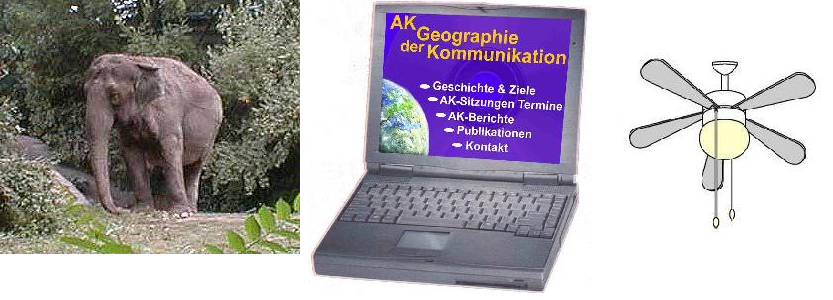
\includegraphics[width=1\linewidth]{caltech.png}
\caption{Ejemplos de imágenes de la base de datos Caltech101. (izq.) Imagen de la clase elephant, (ctro) Imagen de la clase Laptops y (der.) Imagen de la clase celling\_fan}
\end{figure}

\begin{figure}[ht]
\centering
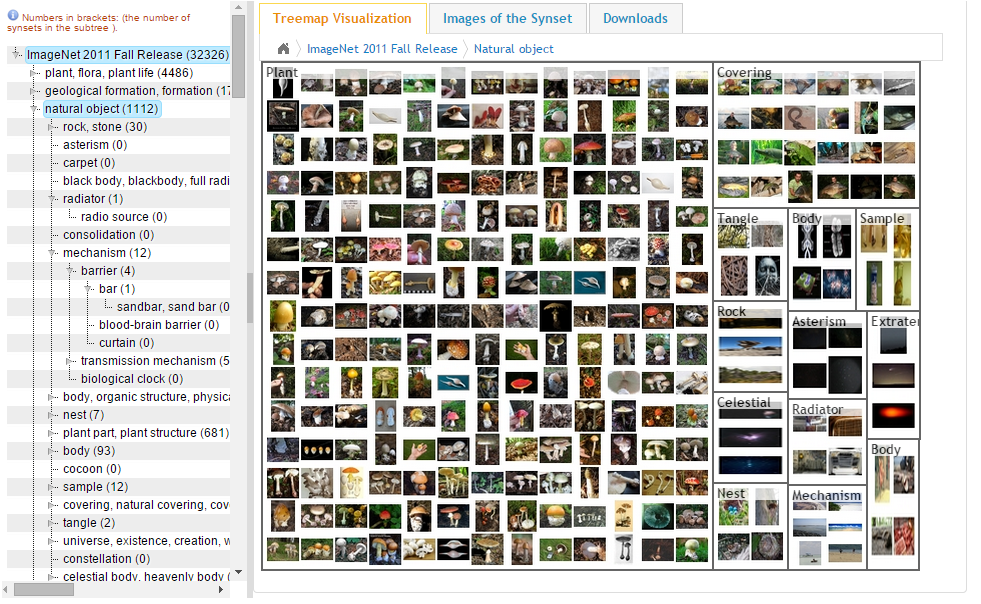
\includegraphics[width=1\linewidth]{BaseDatos.png}
\caption{Base de datos IMAGENET.}
\end{figure}



%------------------------------------------------------------------------
\section{Metodología}

El método de clasificación usa Piryamid Histogram of Words (PHOW), el cual es una versión de SIFT (Scale Invariant Feature Transform), esta función puede rápidamente crear descriptores como bag of words para por detectar una imagen. El método también usa support vector machine con CHI2 para clasificar los descriptores. 
Se usó la librería de vl\_feat. Esta librería contiene algoritmos populares para el tema de visión artificial, los cuales son especializados en entendimiento de imágenes, la localización de características, extracción de información y mapeo (matching) [3]. De esta librería se obtuvo la función PHOW que estaba diseñada a trabajar con la base de datos de Caltech101 con  15 imágenes de entrenamiento por default. 
Las modificaciones del algoritmo para ser uso en la base de datos imagenet-tiny fueron pocas, solo se cambió el directorio de data, se comentó las lineas de codigo para la base de datos Caltech y se cambió el formato de las imágenes .JPEG para que se pudieran extraer en el servidor Guitaca. 
La función phow\_caltech101.m trabaja de la siguiente manera: Primero se obtiene la pirámide de los histogramas de palabras (PHOW) de las imágenes de entrenamiento para obtener un diccionario de palabras (Visual Words). Luego se agrupan en 600 grupos usando kmeans. Posteriormente, se asignan las palabras a cada imagen de entrenamiento. Esta asignación permite entrenar un support vector machine de CHI2. Por último, se evalúan las imágenes construyendo una matriz de confusión y calculando la exactitud (accuracy) como el promedio de aciertos en la diagonal de la matriz de confusión.  
En la Figura 3. se presentan los resultados de phow\_caltech101.m usando la base de datos de Imagenet\_tiny. Con los parámetro del código que están por default. La gráfica de la izquierda corresponde al score que entrega el clasificador a la imagen de test que se evaluó. La imagen de la derecha es la matriz de confusión la cual entrega la exactitud con el promedio de la diagonal dividido entre el número de imágenes de entrenamiento. 

\begin{figure}[ht]
\centering

 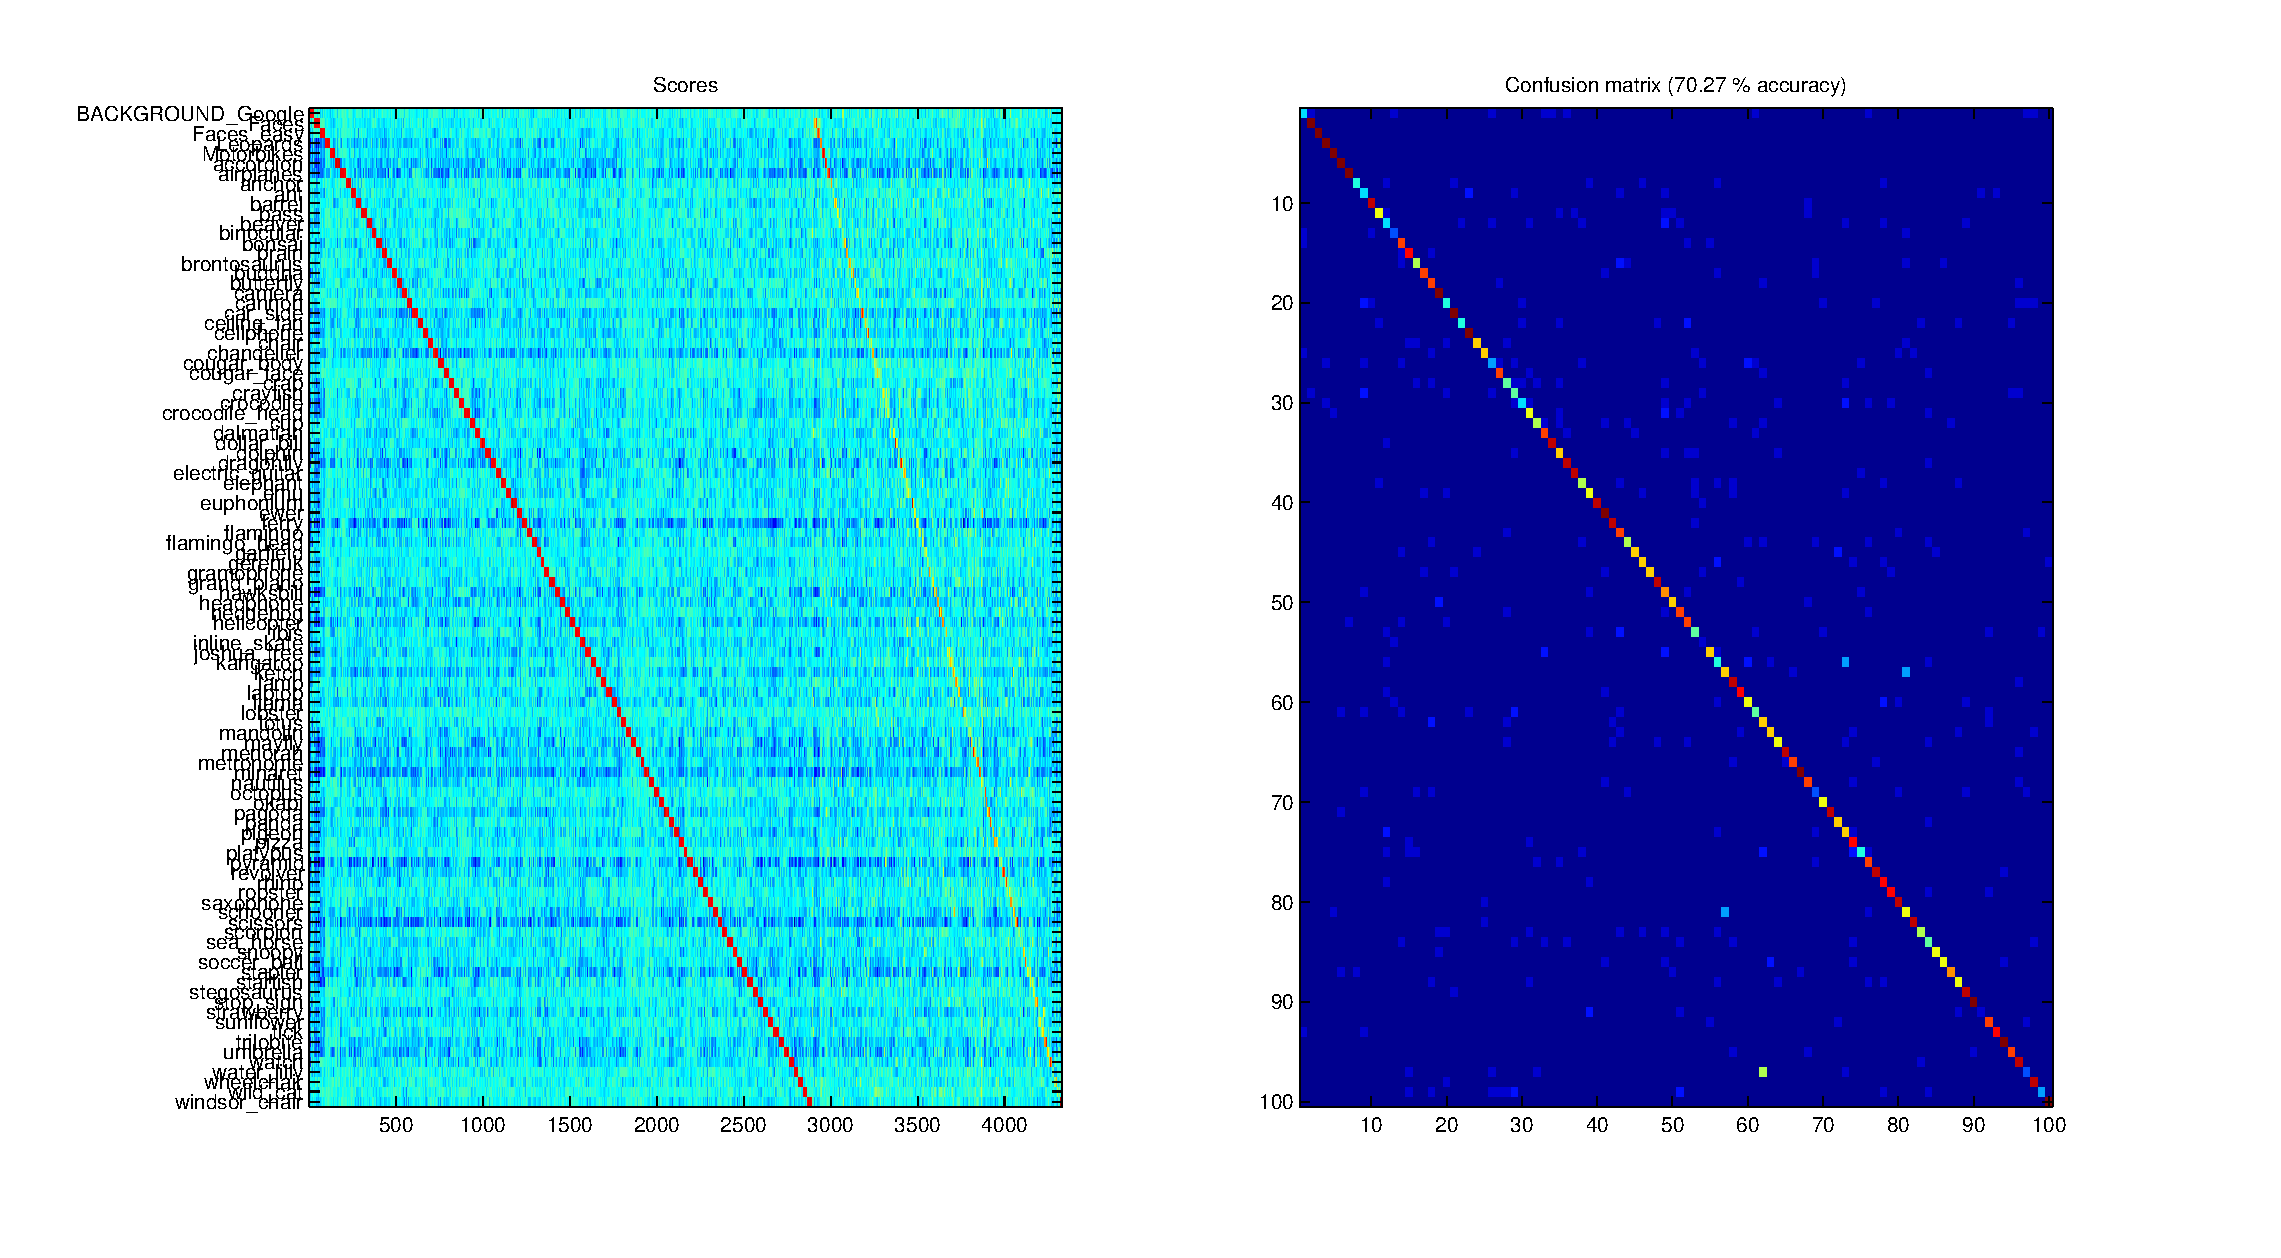
\includegraphics[width=1\linewidth]{Ejemplo_Res_Cal.eps}
\caption{Ejemplo Resultados de la matriz de confusión de phow\_caltech101 con la base de datos de Imagenet\_tiny}
\end{figure}

\subsection{Resultados}

Se midió la exactitud de la matriz de confusión para diferentes combinaciones de los siguientes parámetros:

\begin{itemize}
\item Número de imágenes de entrenamiento: 15, 20, 30, 40 y 80
\item Número de clases: 5, 100. 125, 150 y 200
\item Distancia Espacial x [a b]: a: 1 y 2. b: 1, 2, 4 y 6.
 
 \end{itemize}
 
 
 
Se compararon el método PHOW en las dos bases de datos para diferente número de imágenes de entrenamiento (Ver Figura 4.) con un número fijo de clases de 100, 15 imágenes de test y una distancia espacial x de [2 4].

 \begin{figure}[ht]
\centering

 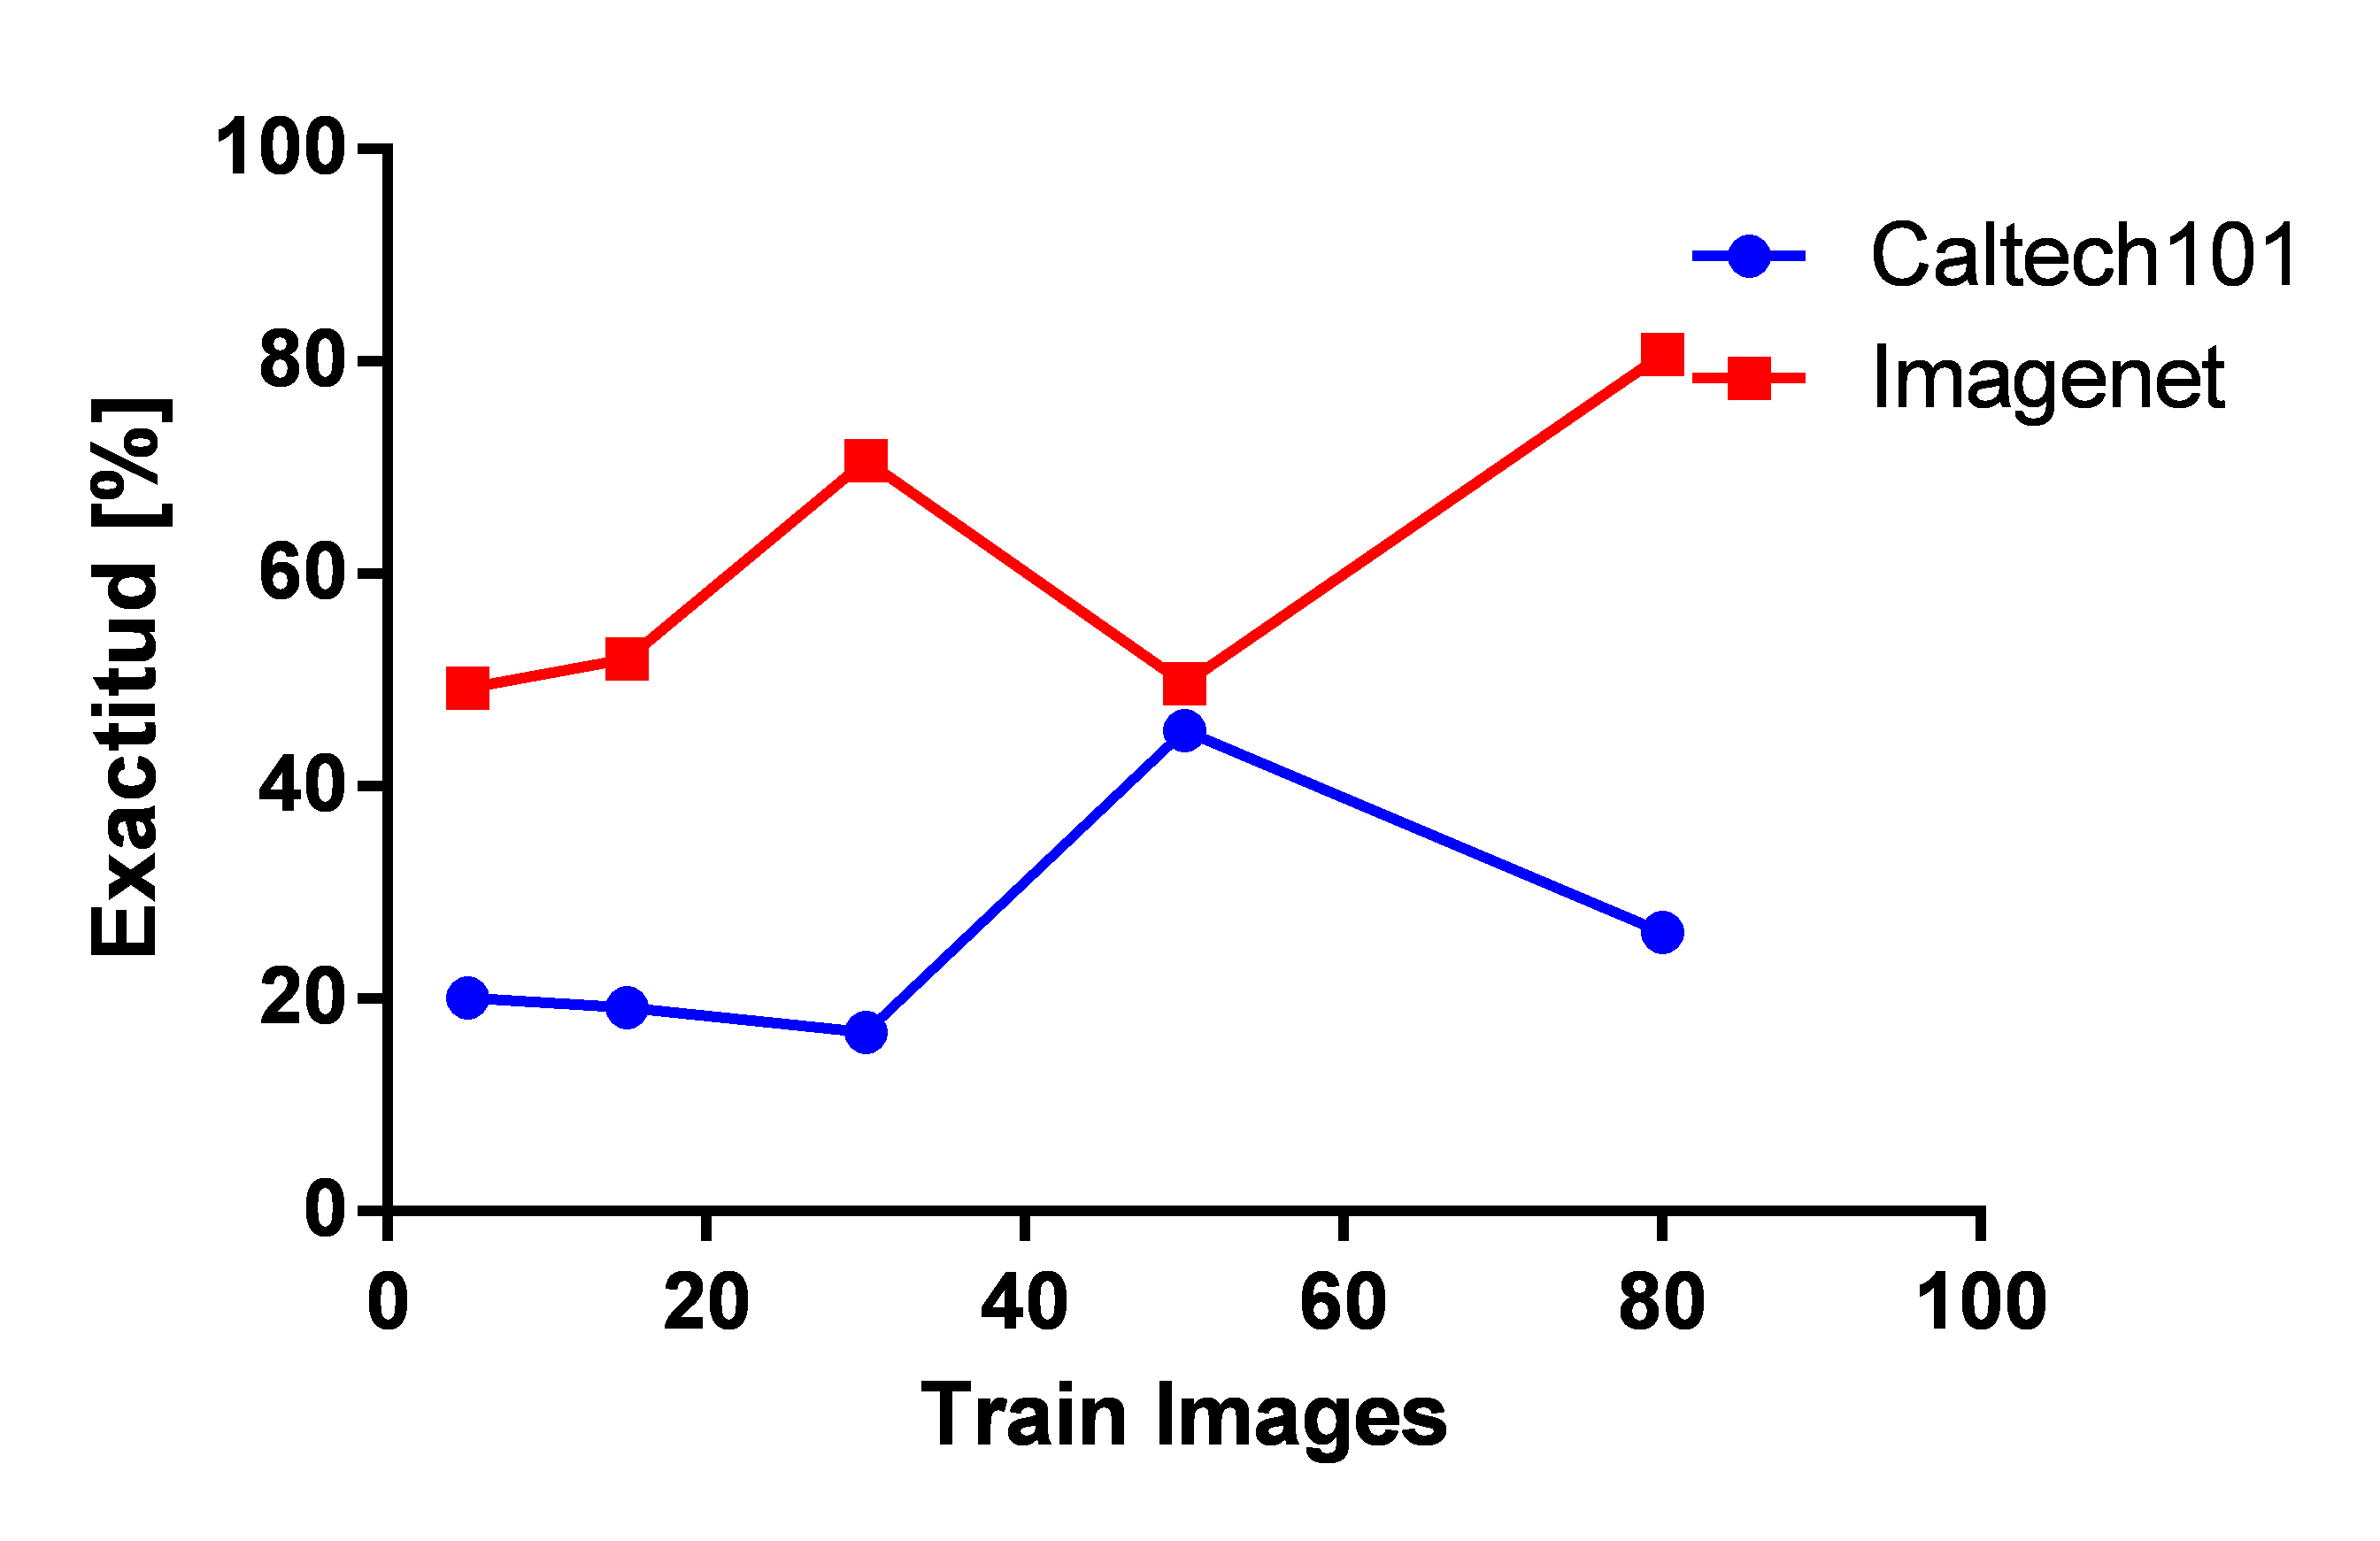
\includegraphics[width=1\linewidth]{calima.png}
\caption{Comparación Bases de datos Caltech101 y Imagenet}
\end{figure}

Se implementaron todas las posibles combinaciones entre el número de clases y el número de imágenes de entrenamiento, se mantuvo constante la distancia espacial x en [2 4] y el número de imágenes de test en 15. Se reporta un total de 25 valores de exactitud (ver Figura 5.). 

\begin{figure}[ht]
\centering
 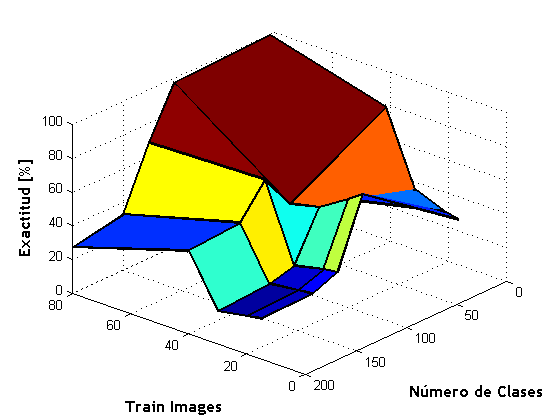
\includegraphics[width=1\linewidth]{resultado__1_.png}
 \caption{Exactitud del método para diferentes número de imágenes de entrenamiento y de clases}
\end{figure}

Por otro lado se mantuvo fijo el valor de clases a 100, el número de imágenes de entrenamiento y de test en 20 y se varió la distancia espacial con las 8 posibles combinaciones mostradas anteriormente. (ver Figura 6.)

\begin{figure}[ht]
\centering

 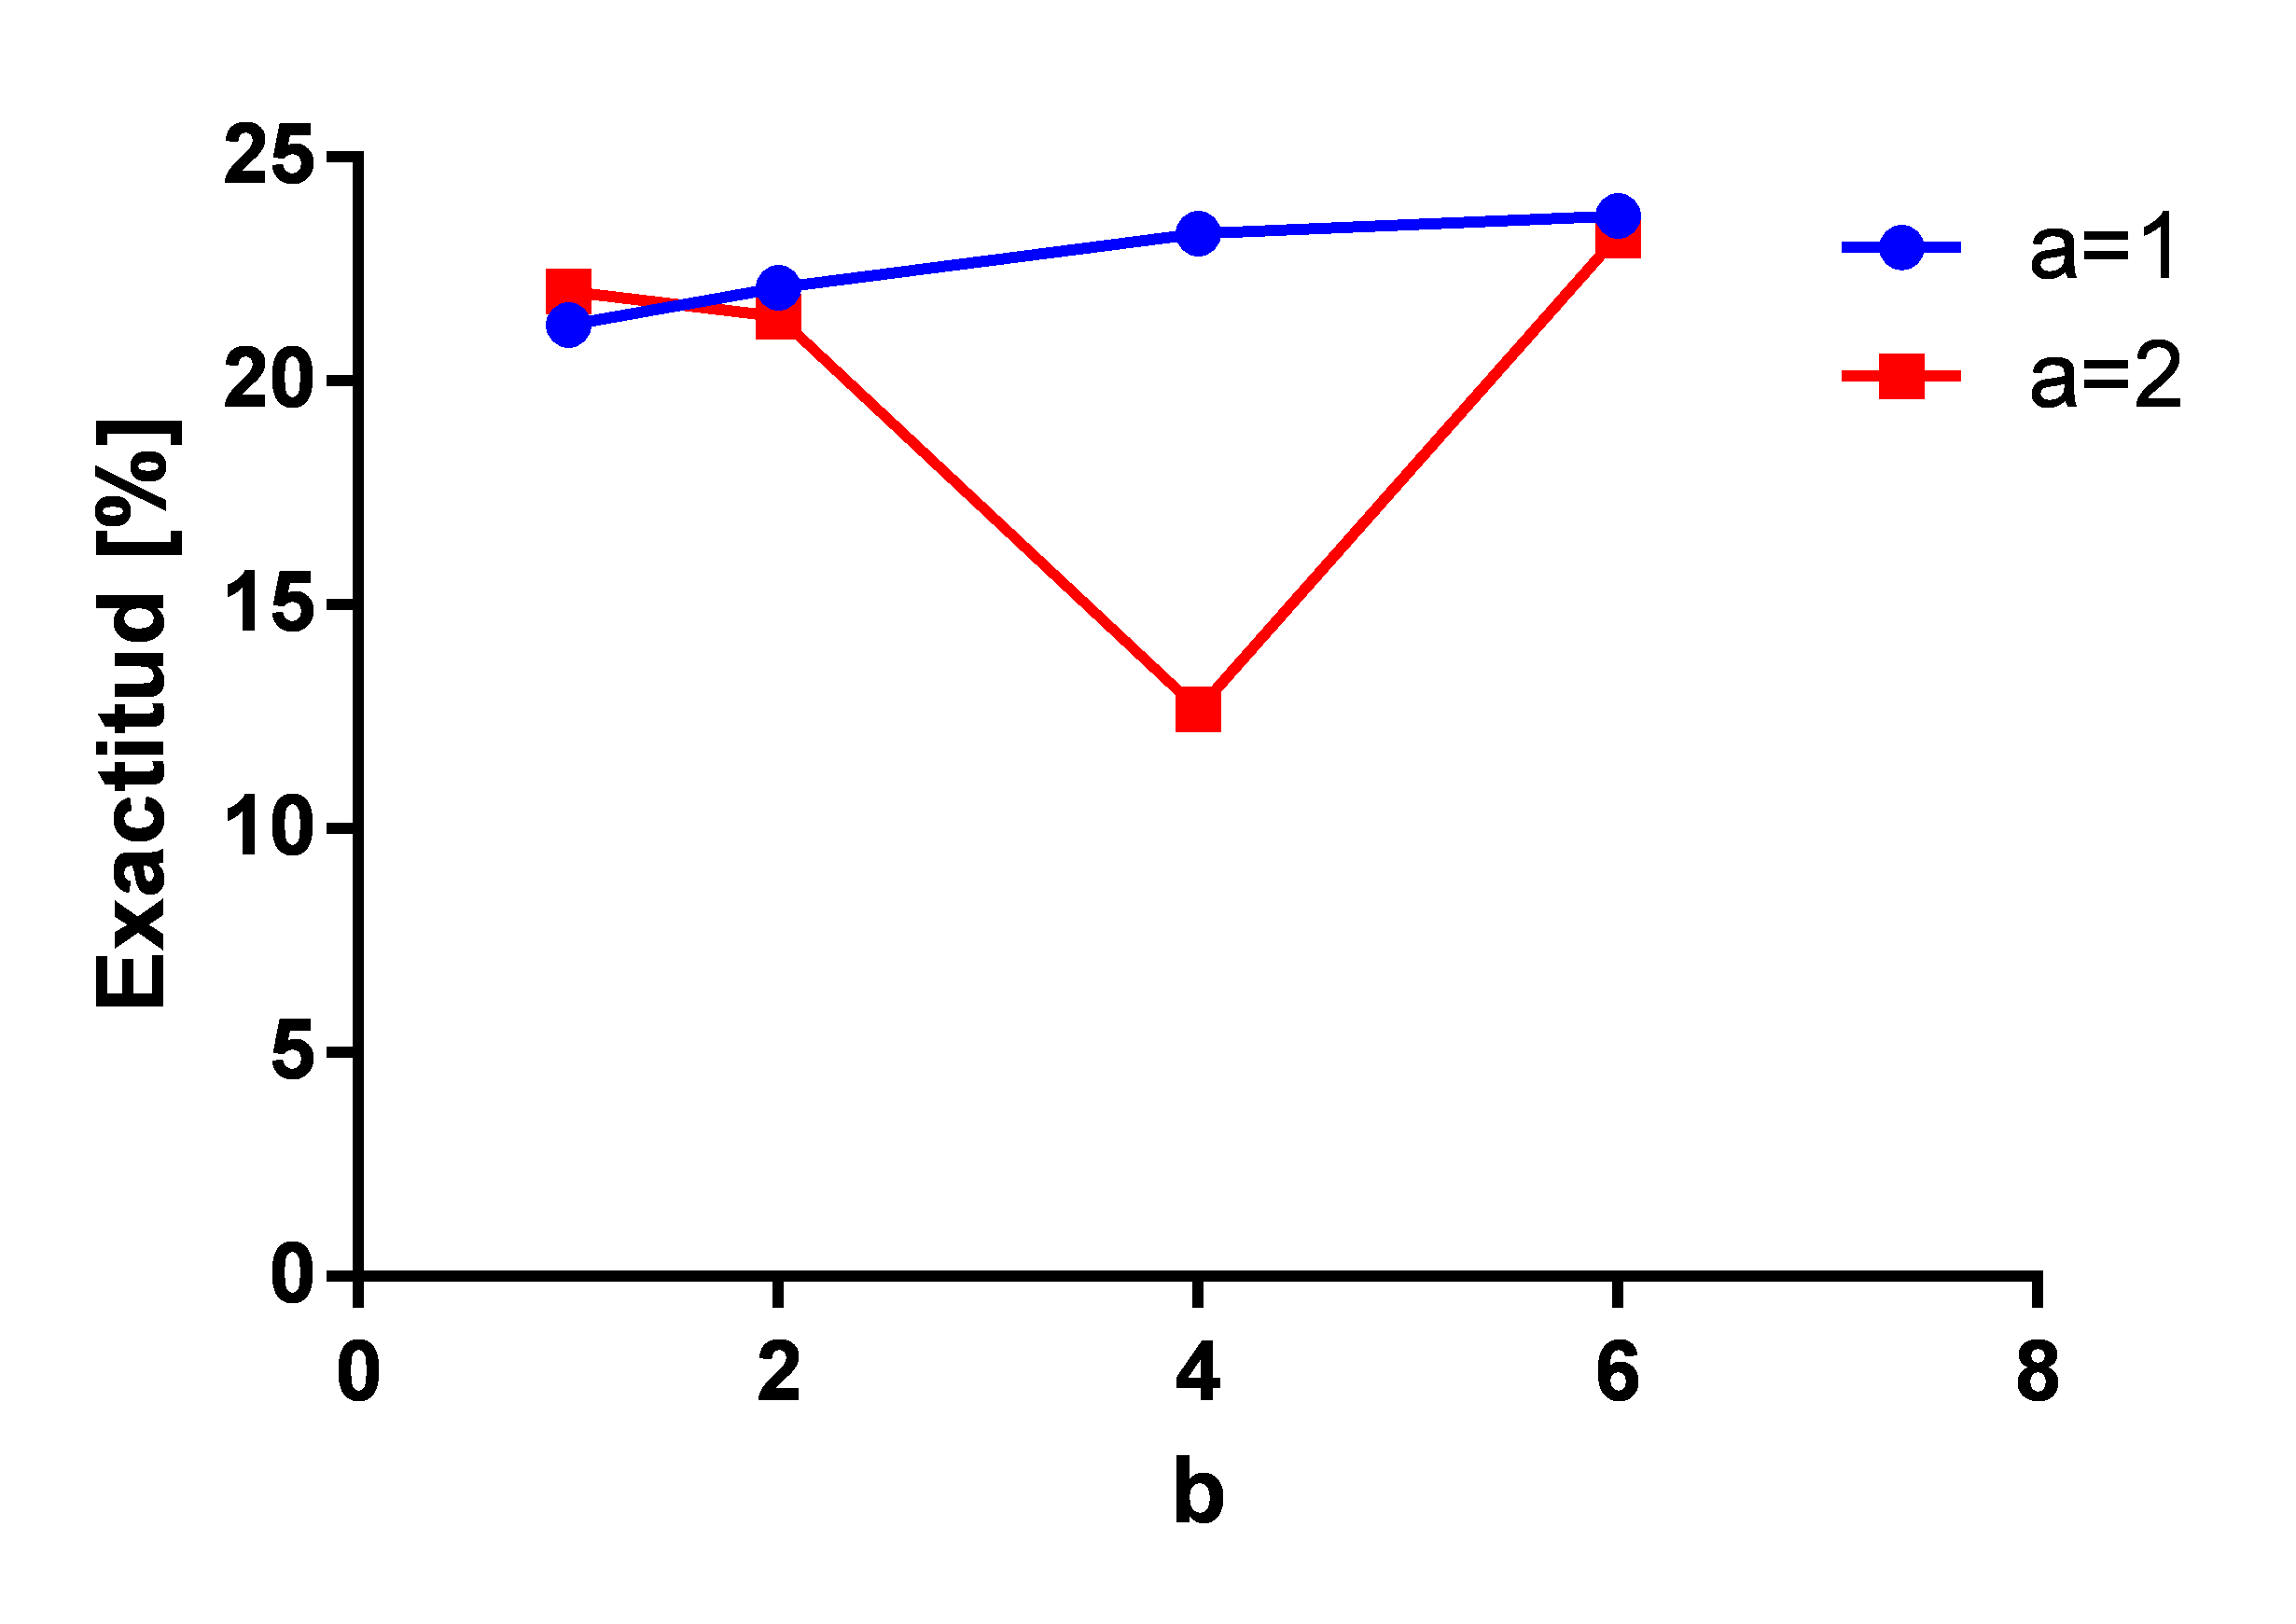
\includegraphics[width=1\linewidth]{AB.png}
 \caption{Exactitud para variación en la distancia espacial x [a b]}

\end{figure}\


También se estudió la variación del número de imágenes de Test para  50 y 100 clases diferentes con 20 imágenes de entrenamiento constante y la distancia espacial x constante en [2 4]. Se estimó la exactitud en cada uno de las combinaciones expuestas anteriormente. 
 
\begin{figure}[ht]
\centering

 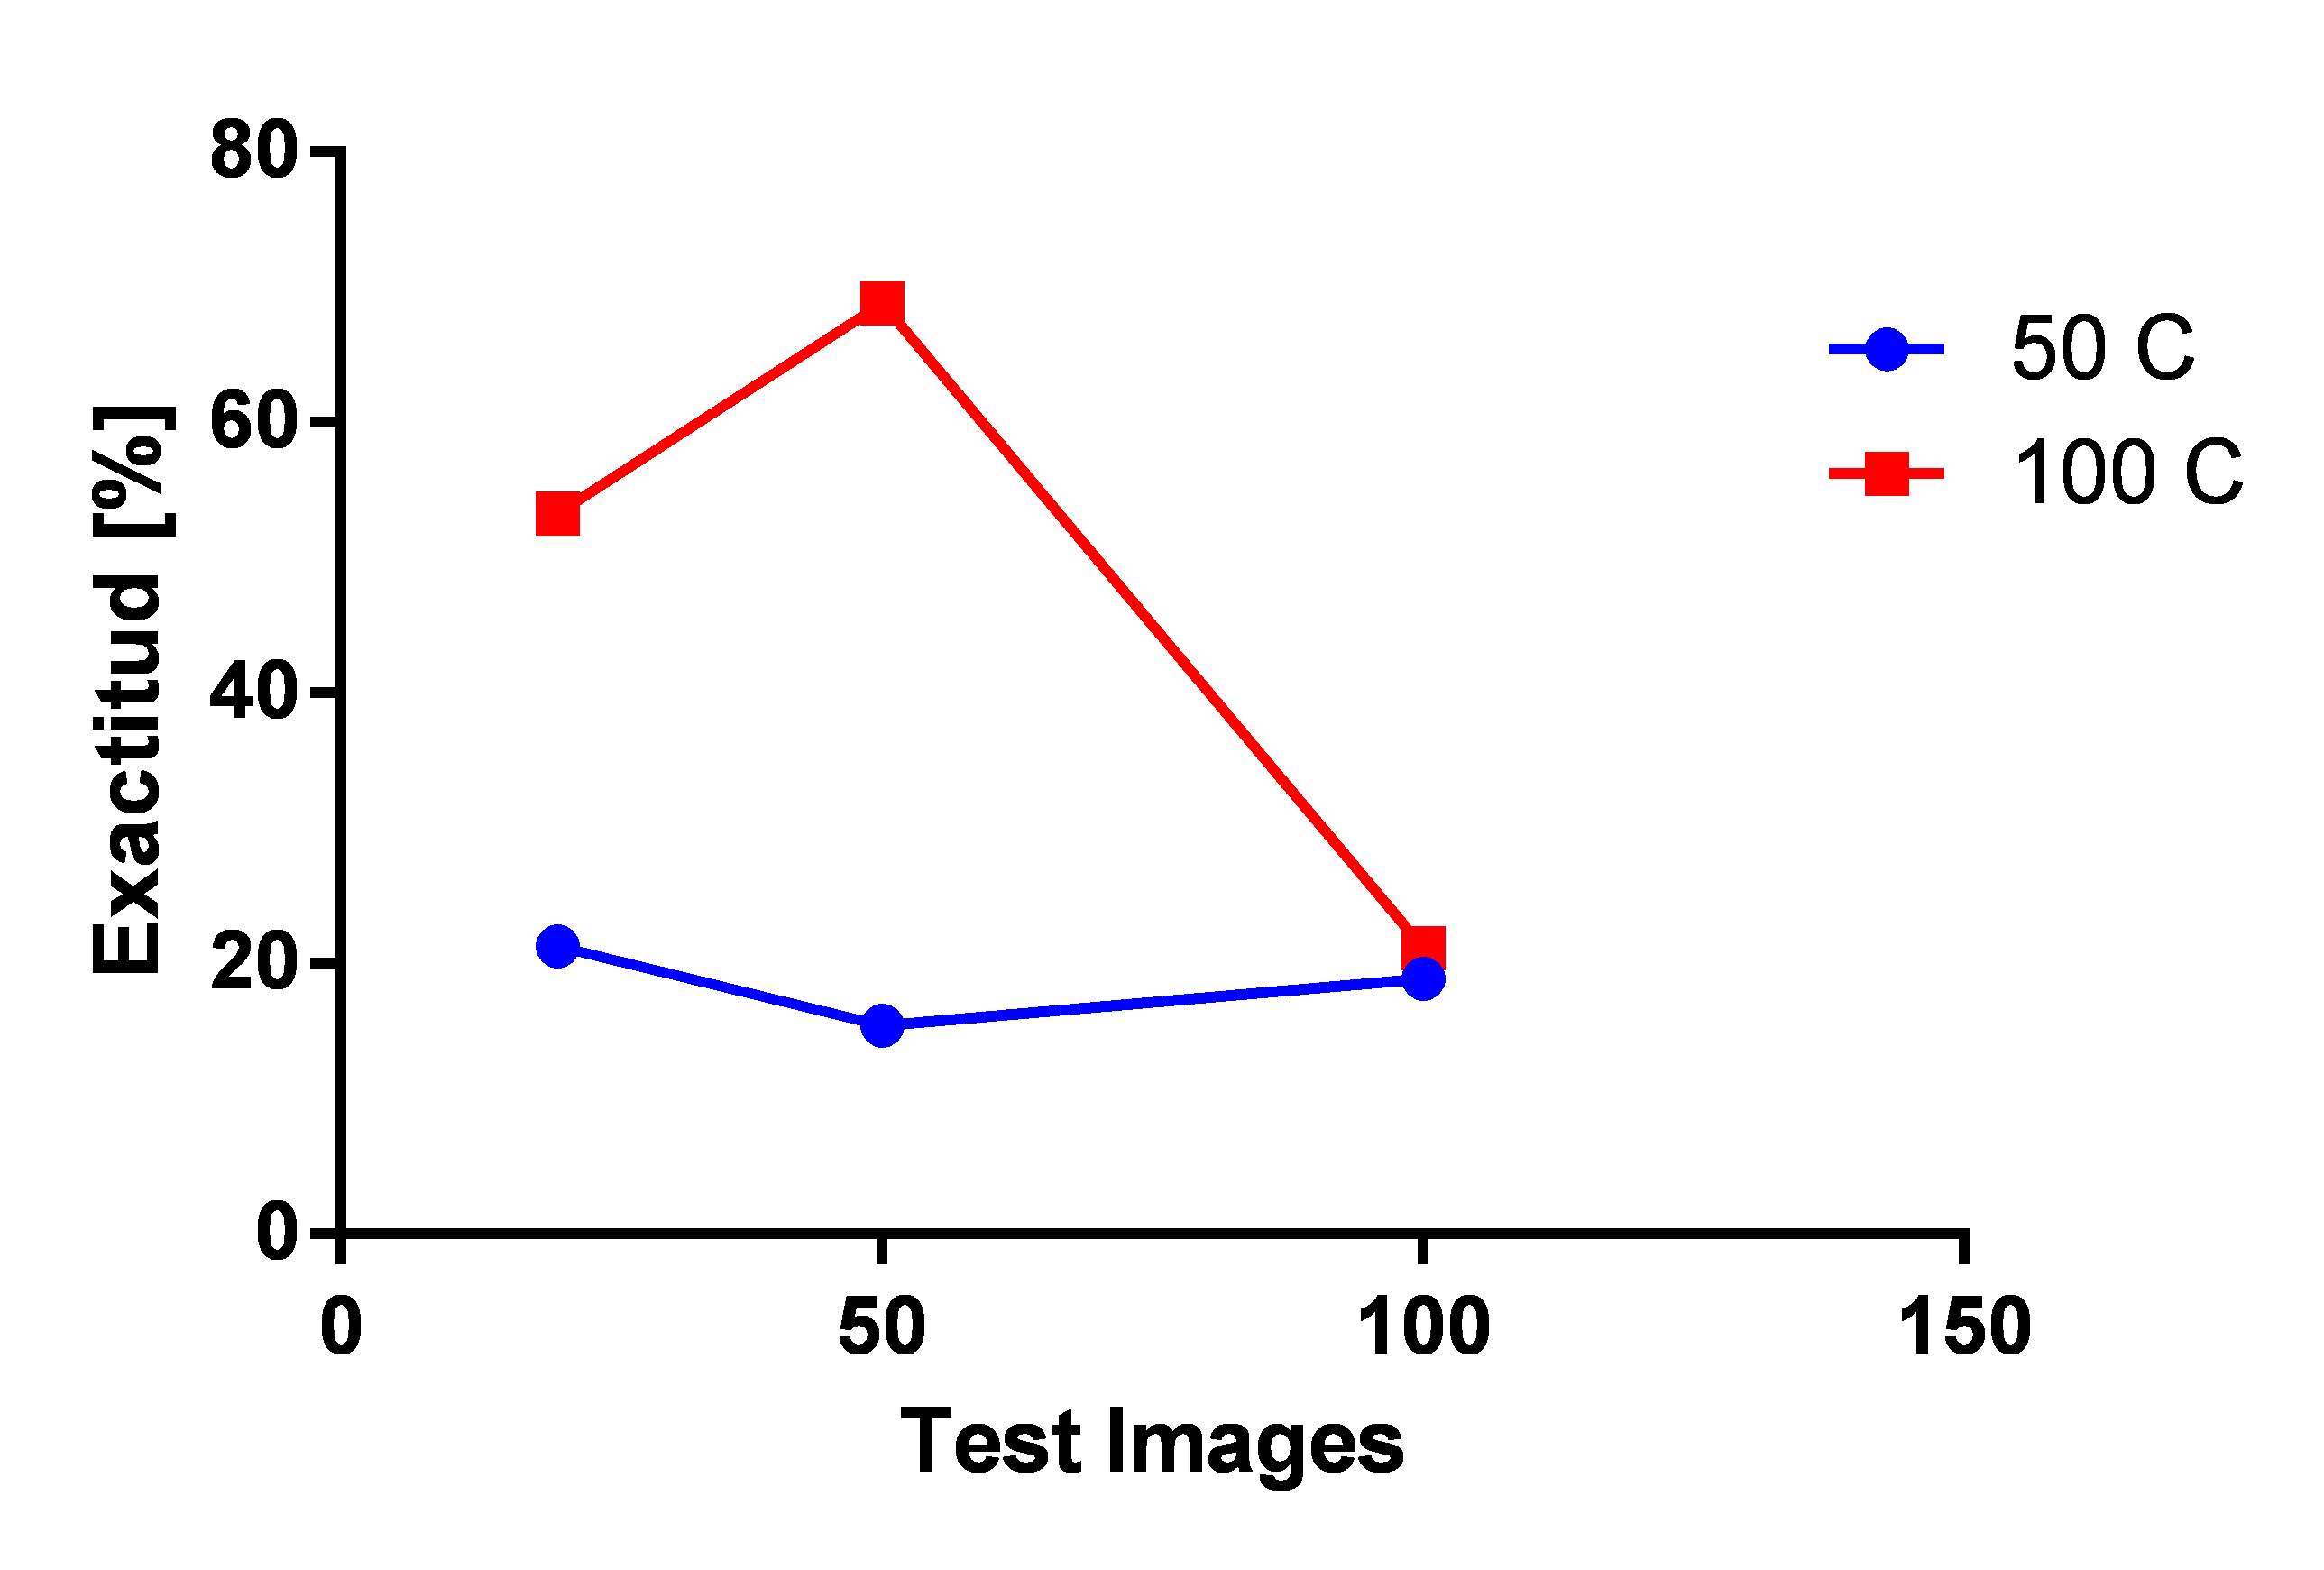
\includegraphics[width=1\linewidth]{Test_images.png}
 \caption{Exactitud para variación del imágenes de Test}

\end{figure}

En general, la mayor exactitud se encontró en la combinación de 5 clases, 80 imágenes de entrenamiento, 15 imágenes de test y una distancia espacial en x de [2 4]. Esta exactitud fue del orden de 96\%, claro que el clasificador con solo 5 clases y 80 imágenes de entrenamiento dará buenos resultados.

Finalmente se estudió el costo computacional en el entrenamiento del SVM y en la evaluación de la matriz de confusión para todas las combinaciones expuestas anteriormente. Se usó la función tic-toc de Matlab. 

\subsection{Análisis de Resultados}

El método PHOW funcionó mejor en la base de datos Imagenet\_tiny con una gran diferencia significativa con 80 imágenes de entrenamiento llegando a valores de 80.7\% mientras que con la base de datos de caltech101 solo se llegó a un valor de exactitud de 26.7\%. Aunque en Caltech101 se llegó a un valor máximo de exactitud de 45\% el cual no es diferente a Imagenet usando 50 imágenes de entrenamiento. 

Vale la pena enfatizar y es que si aumentan las imágenes de evaluación, se baja la exactitud significativamente a valores menores de 20\%.

Se presenta el costo computacional del entrenamiento y del test para la variación del número de imágenes de entrenamiento, número de clases y variación de la distancia espacial en x (ver Figura 7. 8. y 9., respectivamente)

\begin{figure}[ht]
\centering

 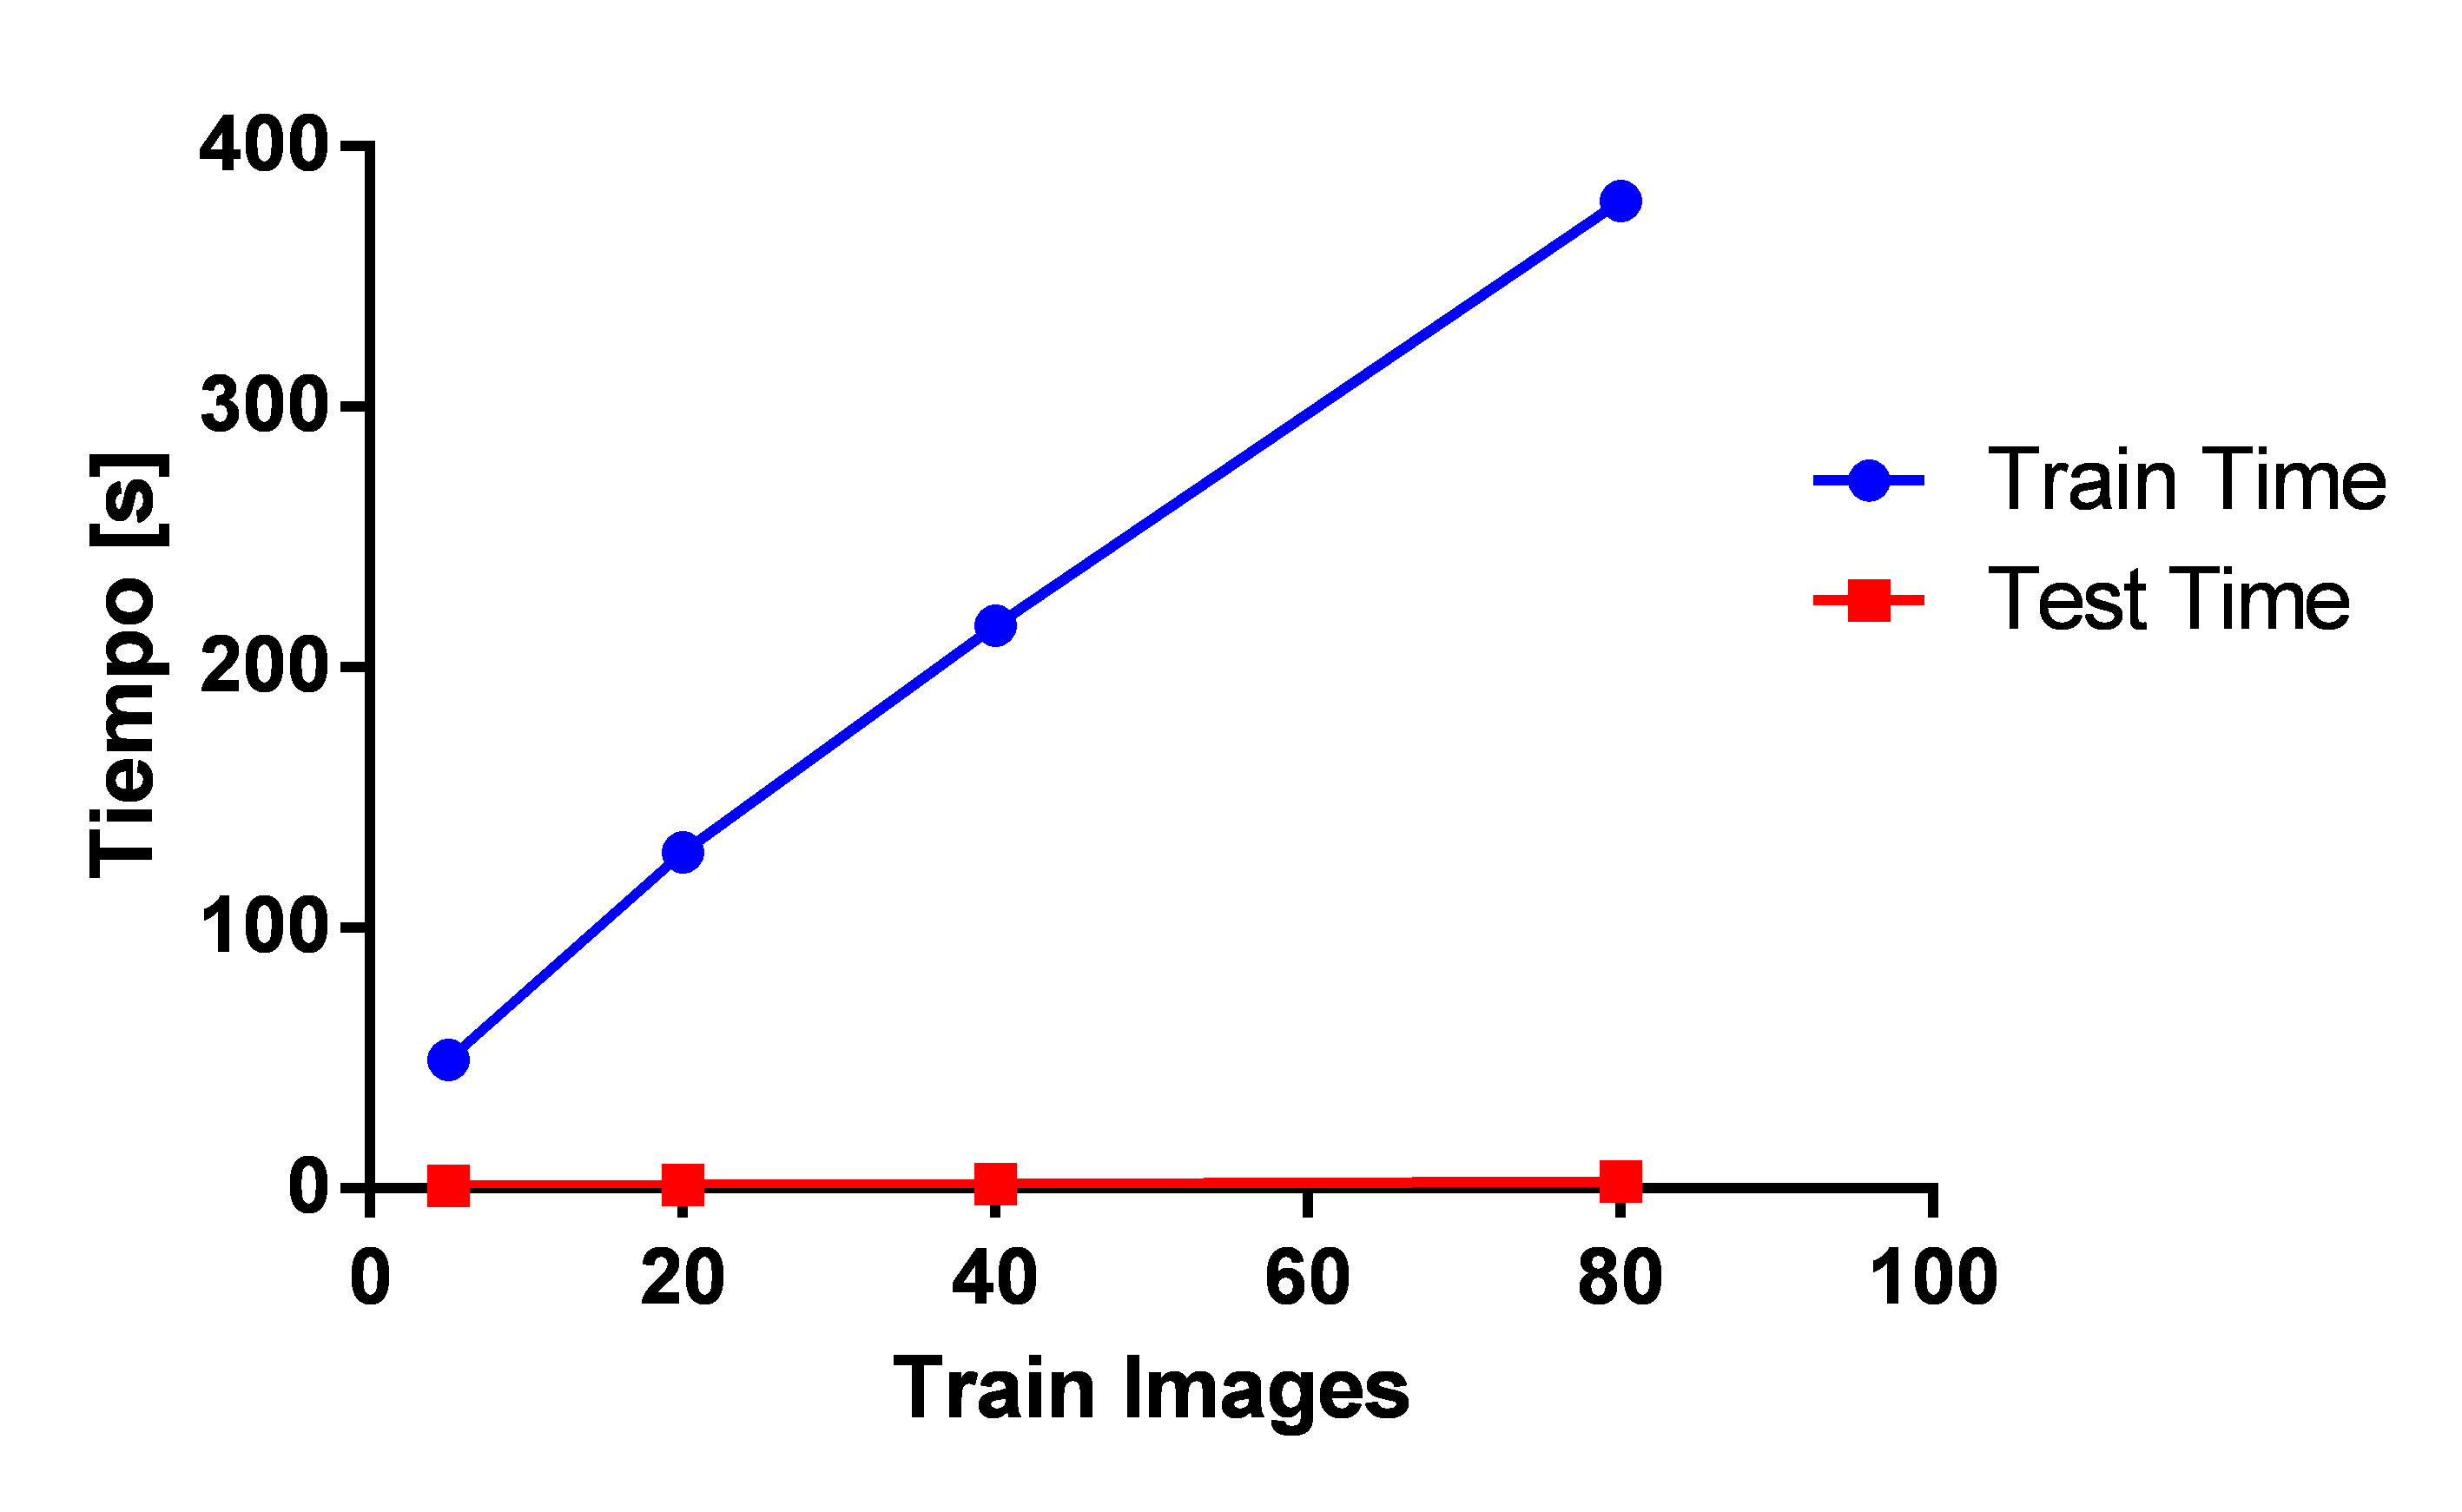
\includegraphics[width=1\linewidth]{Time_Color_Train.png}
\caption{Costo computacional para la variación del número de imágenes de entrenamiento}
\end{figure}

\begin{figure}[ht]
\centering

 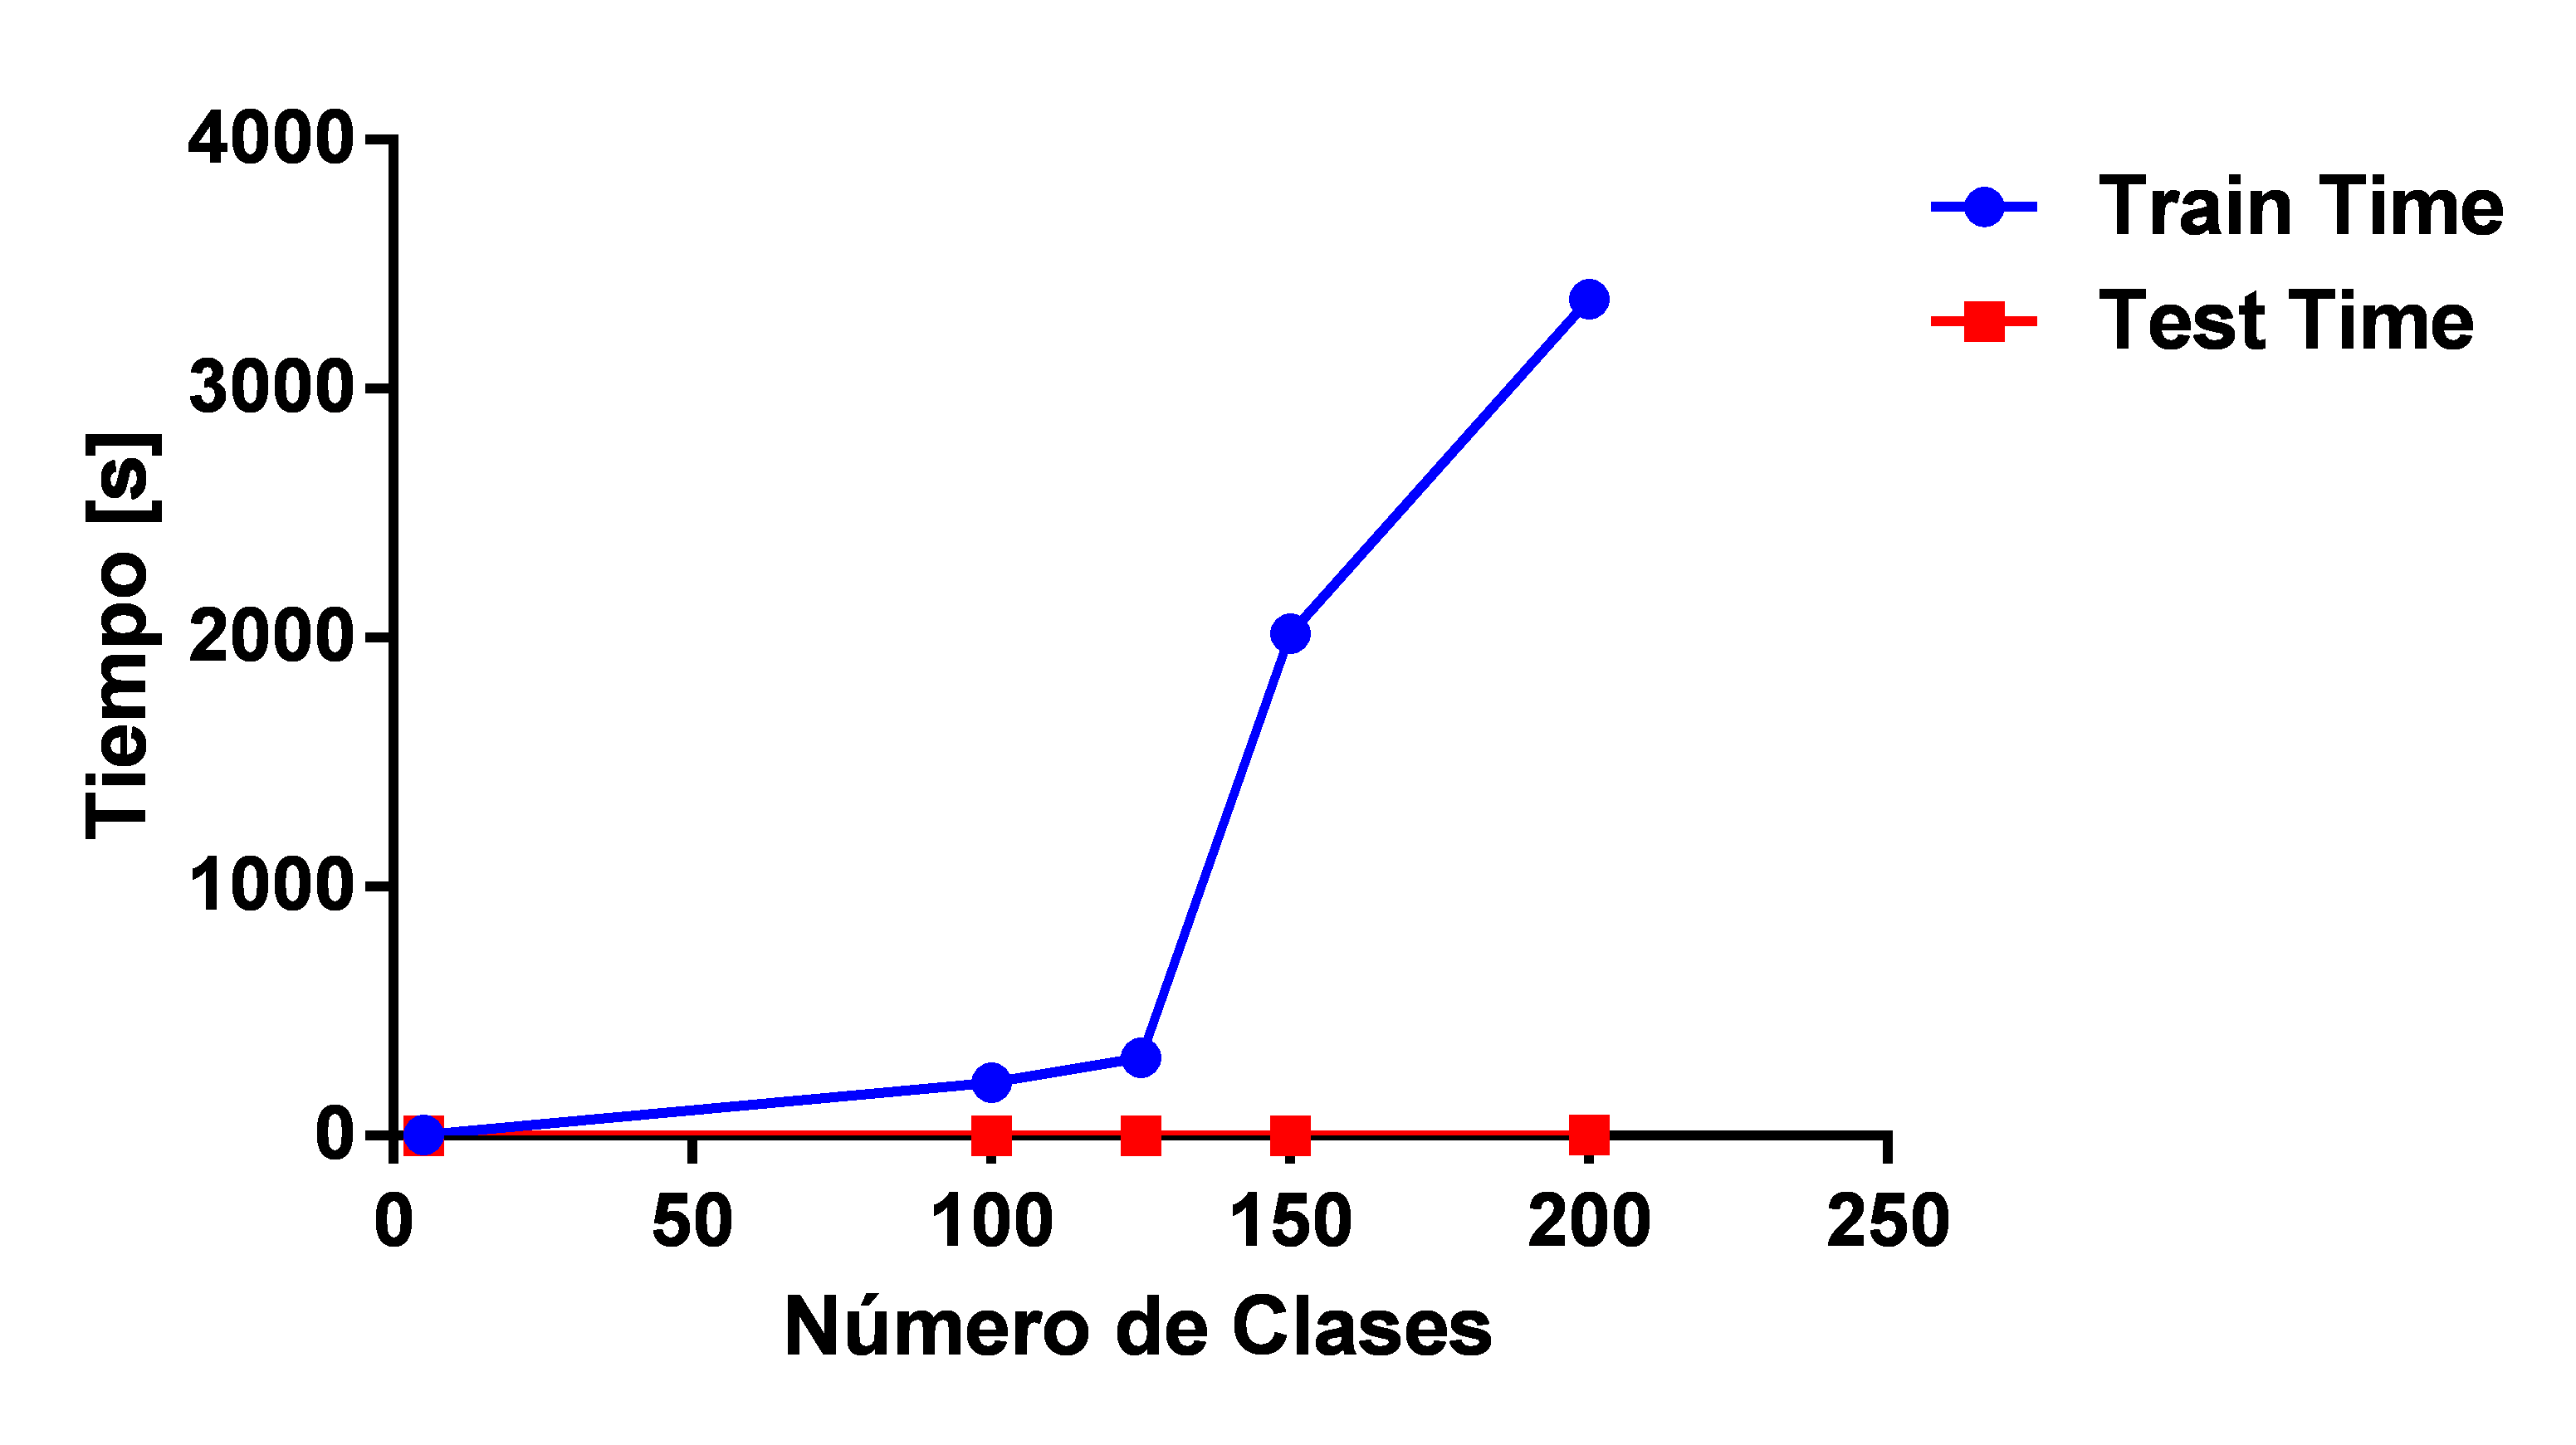
\includegraphics[width=1\linewidth]{Time_Color_classes.png}
\caption{Costo computacional para la variación del número de clases}
\end{figure}
\begin{figure}[ht]
\centering
 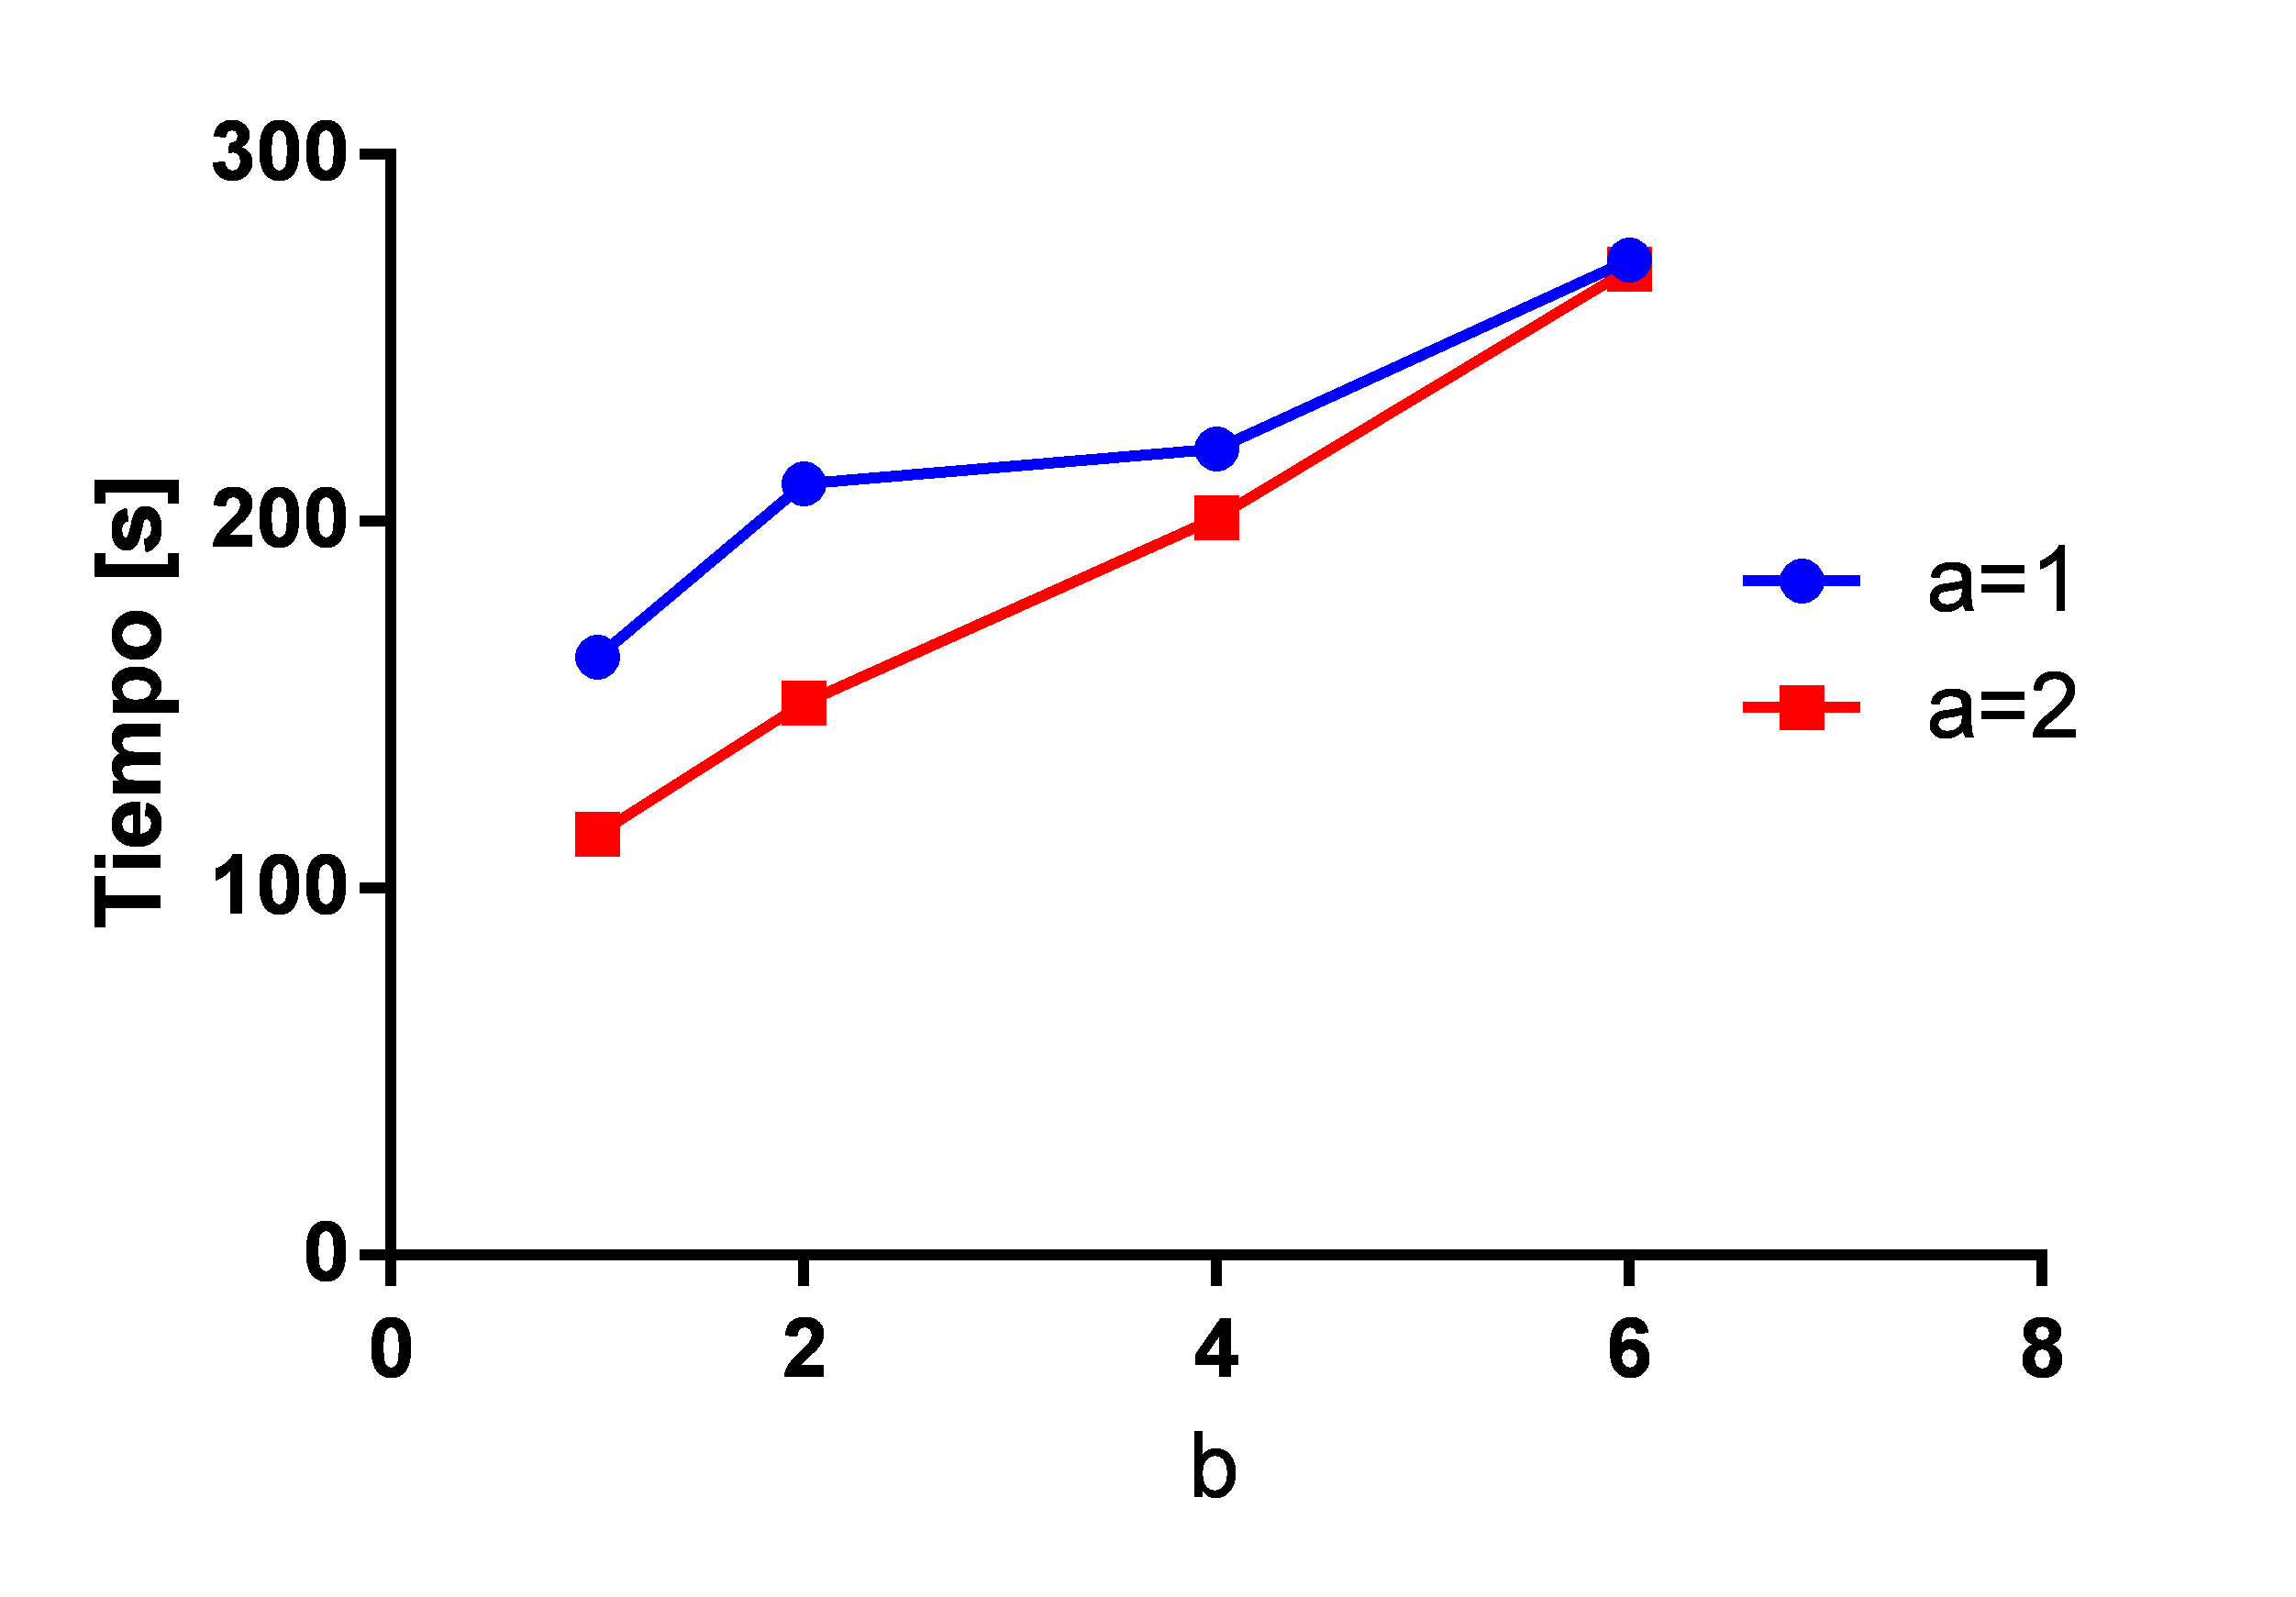
\includegraphics[width=1\linewidth]{Dist_time.png}
\caption{Costo computacional para la variación de la distancia espacial x}
\end{figure}

En la variación de imágenes de entrenamiento, se debe construir un modelo de bag of words mucho más robusto. Esto hace que el tiempo de evaluación aumente casi 4 veces entre 5 imágenes de entrenamiento a 80. Aún así la exactitud logra aumentar casi en un 30\%. En cambio aumentando el número de clases, el costo computacional aumenta en tres ordenes de magnitud y la exactitud disminuye casi a un 20\%. 
Por el lado de la variación de la distancia espacial en x, se encontró que el costo computacional casí se duplica con el cambio de [1 1] a [1 6] o de [2 1] a [2 6], entre el cambio del primer valor de la distancia x no hay diferencia significativa, pero al variar el segundo termino si se encuentra gran diferencia significativa en el costo computacional. Pero esta variación no afecta significativamente la exactitud del método, la mantiene casí entre 20 y 30\%

El costo computacional de test es muy inferior al de entrenamiento. En general es de solo máximo 2 segundos. entrenar el SVM requiere métodos más complejos a medida que aumentan las imágenes de entrenamiento y el número de clases.

En general el aumento de 5 a 200 clases aumenta de 3 a 3500 segundos el costo computacional de entrenamiento y disminuye la exactitud a valores de 20\%. Entre más imagenes de test, también disminuye la exactitud. La distancia espacial en x casí no genera cambios en la exactitud.  

\section{Limitaciones y Posibles Mejoras}

El método de SIFT está diseñado para bases de datos más sencillas. Aunque se encontró que en imagenet funciona bien. Pero si se aumentan las clases a las 200 de imagenet\_tiny, el método no funciona bien con valores de exactitud de 20\%. Se propone mejorar SIFT añadiendo mejores métodos que tengan en cuenta deformación de objetos y penalicen por energías las posiciones incorrectas de un objeto. También SVM con CHI2 es muy limitante, se podría encontrar una mejor manera de entranmiento sin tanto costo computacional. 

\section{Referencias}

\begin{quote}
   
[1] L. Fei-Fei, R. Fergus, and P. Perona.  Learning generative visual models from few training examples: an incremental Bayesian approach tested on 101 object categories. CVPR 2004, Workshop on Generative-Model Based Vision. 2004
   
   [2] L. Fei-Fei and O. Russakovsky, Analysis of Large-Scale Visual Recognition, Bay Area Vision Meeting, October, 2013
   
   [3] A. Vedaldi and B. Fulkerson, (VLFeat)\: An Open and Portable Library of Computer Vision Algorithms.2008. 
    
   
\end{quote}

{\small
\bibliographystyle{ieee}
\bibliography{egbib}
}




\end{document}
